% Presentation-only derivative; scripts/build_appendix_compact_tables_20261106.py
\begin{figure}[!htbp]
\centering
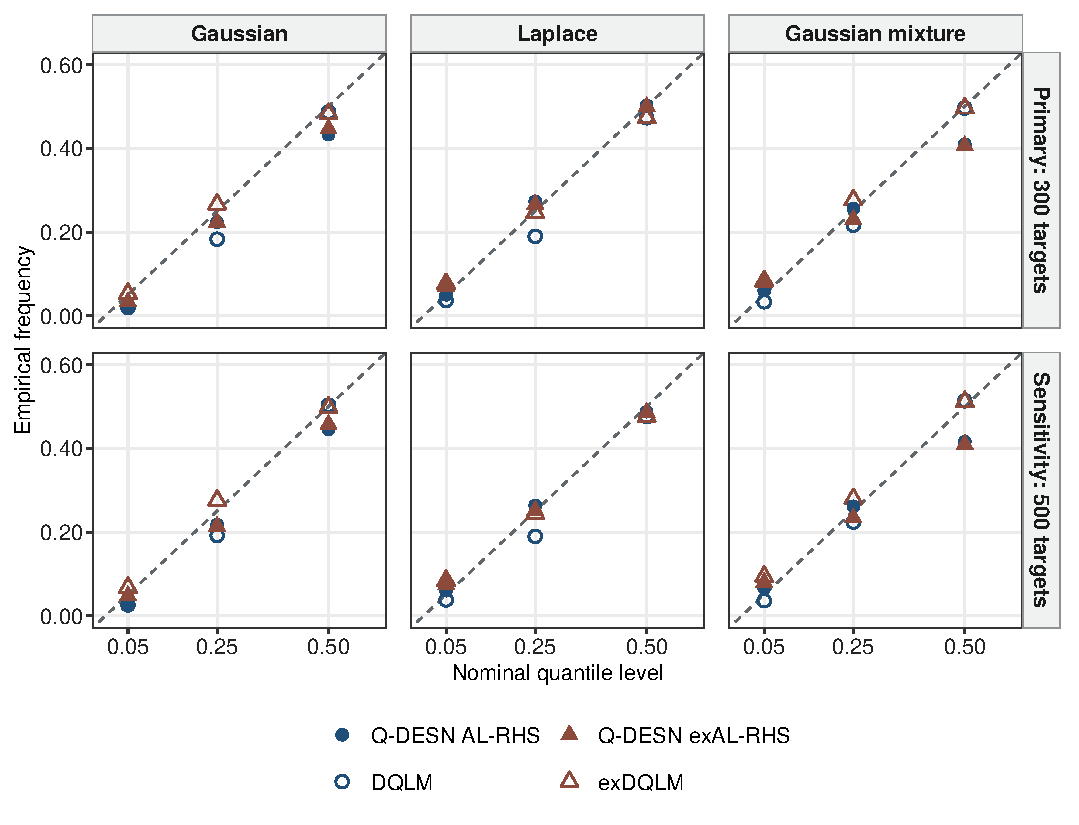
\includegraphics[width=0.98\textwidth]{figures/independent_simulation/independent_forecast_calibration_v1.pdf}
\caption{Empirical quantile frequencies over 300 and 500 targets using the check-loss specifications and pooled posterior-median forecasts. Each level uses its quantile-centred response series. Colours and symbols follow Figure~\ref{fig:simulation-500obs-mcmc-forecast-mae-intervals}; the dashed diagonal is nominal. No sampling confidence bands are shown.}
\figalt{Six panels compare empirical response frequencies below posterior-median quantile forecasts with the nominal levels 0.05, 0.25 and 0.50, for four models, three error families and two evaluation periods.}
\label{fig:supp-independent-quantile-calibration}
\end{figure}
